\documentclass[a4paper,10pt]{article}

\usepackage{amsmath}
\usepackage{amssymb}
\usepackage{amsthm}
\usepackage[hangul]{kotex}
\usepackage{graphicx}
\usepackage{multirow}
\usepackage{dsfont,pifont,amssymb}
\usepackage{pict2e}
\usepackage{float}

\newtheorem{prob}{Problem}

\graphicspath{{images/}}
\begin{document}
\title{GSHS Discrete Data Structures Assignment \#1}
\author{Author : 14080 Sangheon Lee}
\date{}
\maketitle
\begin{prob}
	눈금이 없는 직각삼각자와 연필만 가지고 주어진 원의 중심을 찾을 수 있겠는가?
\end{prob}
매우 간단한 문제이다. 원 내의 지름을 빗변으로 가지는 삼각형은 직각삼각형임을 이용하면, 원주 위의 임의의 점 하나를 잡아, 직각삼각자의 직각 부분을 이용하여 선을 긋는다. 이 때 원주와 생기는 교점 2개를 이으면 지름이 생기며, 이를 다른 점에 대해 한 번 더 하면 지름들의 교점이 생기고, 이는 곧 원의 지름이다.\\
\begin{prob}
	어떤 빌딩의 1층에서 꼭대기 층까지 엘리베이터를 타고 제일 꼭대기 층까지 가기 위해 기다리고 있다. 그런데 이 엘리베이터는 운반할 수 있는 최대 중량은 300kg이고 엘리베이터를 작동하기 위해서는 세 명 중 한 명은 반드시 엘리베이터를 타고 있어야 한다. 이들 중 3명의 무게가 각각 130kg, 160kg, 210kg일 때, 그들이 꼭대기 층까지 엘리베이터를 타고 갈 수 있을까? 갈 수 있다면 방법을 말하라.
\end{prob}
가능하다. 다음 표를 보라.
\begin{table}[H]
	\centering
	
	\label{my-label}
	\begin{tabular}{|c|c|c|}
		\hline
		Ground        & Elevator                             & Top           \\ \hline
		130, 160, 210 &                                      &               \\ \hline
		210           & -\textgreater 130, 160 -\textgreater &               \\ \hline
		210           &                                      & 130, 160      \\ \hline
		210           & \textless- 130 \textless-            & 160           \\ \hline
		130, 210      &                                      & 160           \\ \hline
		130           & -\textgreater 210 -\textgreater      & 160           \\ \hline
		130           &                                      & 160, 210      \\ \hline
		130           & \textless- 160 \textless-            & 210           \\ \hline
		130, 160      &                                      & 210           \\ \hline
		& -\textgreater 130, 160 -\textgreater & 210           \\ \hline
		&                                      & 130, 160, 210 \\ \hline
	\end{tabular}
	\caption{문제 2의 정답}
\end{table}
\begin{prob}
	흔한 병에 적당한 양의 물이 들어가 있다. 물을 더하거나 붓지 않고 자(ruler)만으로 병의 부피를 측정하는 것이 가능한가? 가능하다면 방법을 설명하라.
\end{prob}
우선 물의 부피를 자를 이용해 잰 다음에, \textbf{병을 뒤집어서} 공기의 부피를 자를 이용해 잰 다음 더하면 된다. Wow!
\begin{prob}
	오른쪽 그림의 시계의 앞면을 두 직선으로 나눌 때, 각 영역의 있는 숫자들의 합이 같도록 나눌 수 있겠는가? 또, 각 영역이 두 수를 포함하고 이 두 수의 합이 같도록 6개의 영역으로 나눌 수 있겠는가?
\end{prob}
일단 첫번째 sub-task부터 생각해보자. 직선을 배치하는 경우는 다음 두 가지 중 하나이다.
\begin{enumerate}
	%\item[1.] 두 직선이 일치해서 구역이 2개로 나누어지는 경우
	\item[1.] 두 직선이 일치하지는 않으나 교점이 없어 구역이 3개로 나누어지는 경우
	\item[2.] 두 직선이 교점이 있어 구역이 4개로 나누어지는 경우
\end{enumerate}
각각의 경우에 대해 생각해보면 다음과 같다.
\begin{enumerate}
	%\item[1.] 두 직선이 일치해서 구역이 2개로 나누어지는 경우\\
	%우선 자명한 것을 생각해보자. 구역이 2개로 나누어질 때 한 구역은 $k$개의 수를, 다른 구역은 $12-k$개의 수를 가진다. $min(k, 12-k) \leq 6$이고, 또 어떤 구역이 최대의 합을 가지려면 $12-k+1$부터 $12$까지 더해야 한다. 이렇게 생각하면 $k\leq 3$일 때는 답이 없다.\\
	%또, $k=4$일 때는 최대가 $9+10+11+12=42$이고 그 다음은 $8+9+10+11=38$이여서 답이 없고, $ k=5 $일 때는 $ 12 $와 $ 1 $을 동시에 가지지 않으면 5의 배수이니 아니고, $ 12 $와 $ 1 $을 동시에 가지는 경우는 최대가 $ 9+10+11+12+1=43 $이고 그 다음이 $ 10+11+12+1+2=36 $이므로 답이 없다.\\
	%마지막으로 $k=6$일 때는 거두절미하고, $4+5+6+7+8+9=10+11+12+1+2+3=39$이며, 이 경우가 유일하다.
	
	\item[1.] 두 직선이 일치하지는 않으나 교점이 없어 구역이 3개로 나누어지는 경우\\
	이 때 각 구역의 합은 $ 78/3=26 $이 되어야 한다. 일단 수가 분리되어 있지 않고 연속($ 12,\ 1 $도 포함)되어 있는 구역이 적어도 하나는 존재하므로 이를 구해보자.\\
	구역에 있는 수가 2개 이하면 최대값이 $ 23 $이여서 답이 없고, 3개면 어떻게 해도 합이 3의 배수가 되어 답이 없다. 4개이면 $ 12,\ 1 $을 포함하지 아닐 경우 4의 배수여서 아니고, $ 12,\ 1 $을 포함한 경우	$11+12+1+2=26$과 $5+6+7+8=26$인 때가 유이한 답이다.\\
	5개에 있는 경우는 $ 12,\ 1 $을 포함하지 않을 경우 합이 5의 배수이니까 아니고, 포함하더라도 만족하는 경우는 없다. 마찬가지로 6개일 때도 없고, 7개 이상일 때는 최소값이 28이 되어 counting이 끝난 것을 알 수 있다.
	즉 이 때 답은 $(11,12,1,2),(3,4,9,10),(5,6,7,8)$이다.
	
	\item[2.] 두 직선이 교점이 있어 구역이 4개로 나누어지는 경우\\
	78은 4의 배수가 아니다. 그러므로 이런 경우는 없다. 끝.
\end{enumerate}
두 번째 sub-task는 더 간단하다. 합이 13인 여섯 개의 영역을 나누려면 우의 각 영역은 최소 2개의 숫자를 포함해야 한다. 그런데 2*6=12이므로 모든 영역은 수가 2개이다. 그러므로 $(1,12),(2,11),(3,10),(4,9),(5,8),(6,7)$의 형태로 분할할 수 있고 이가 유일하다.
\begin{prob}
	정육면체의 각 꼭짓점에 원이 그려져 있다. 원 안에 1부터 8까지의 수를 적되, 이 정육면체에 모서리에 의해 연결된 두 원 안에 있는 숫자들의 차가 항상 1보다 크게 적어넣는 경우가 가능하겠는가?
\end{prob}
가능하다. 다음 \LaTeX발 그림이 한 예이다. 그냥 그림판으로 만들걸......
\setlength{\unitlength}{.3cm}
\begin{center}
	\begin{picture}(16,16)
		\thicklines
		\put(2,3){\line(0,1){6}}
		\put(10,3){\line(0,1){6}}
		\put(4.8284,5.8284){\line(0,1){6}}
		\put(12.8284,5.8284){\line(0,1){6}}
		\put(2.7071,2.7071){\line(1,1){1.4142}}
		\put(2.7071,10.7071){\line(1,1){1.4142}}
		\put(10.7071,2.7071){\line(1,1){1.4142}}
		\put(10.7071,10.7071){\line(1,1){1.4142}}
		\put(3,2){\line(1,0){6}}
		\put(3,10){\line(1,0){6}}
		\put(5.8284,4.8284){\line(1,0){6}}
		\put(5.8284,12.8284){\line(1,0){6}}
		
		\put(2,2){\circle{2}}
		\put(2,10){\circle{2}}
		\put(10,2){\circle{2}}
		\put(10,10){\circle{2}}
		\put(4.8284,4.8284){\circle{2}}
		\put(4.8284,12.8284){\circle{2}}
		\put(12.8284,4.8284){\circle{2}}
		\put(12.8284,12.8284){\circle{2}}
		
		\put(4.5284,12.4784){$\displaystyle 3$}
		\put(12.5284,12.4784){$\displaystyle 8$}
		\put(1.7,9.65){$\displaystyle 5$}
		\put(9.7,9.65){$\displaystyle 2$}
		\put(4.5284,4.4784){$\displaystyle 7$}
		\put(12.5284,4.4784){$\displaystyle 4$}
		\put(1.7,1.65){$\displaystyle 1$}
		\put(9.7,1.65){$\displaystyle 6$}
	\end{picture}
\end{center}
\begin{prob}
	흰 바북돌 3개, 검은 바둑돌 3개가 그림과 같이 칸 안에 놓여 있다. 바둑 돌을 바로 옆에 있는 빈 칸이나 바로 옆에 있는 바둑돌을 뛰어 넘어 빈 칸으로 옮기는 시행을 여러 번 반복하여, 흰 바둑돌을 오른쪽으로, 검은 바둑돌을 왼쪽으로 모을 수 있겠는가?\\
	\begin{figure}[h]
		\begin{center}
			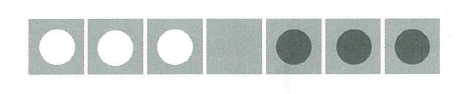
\includegraphics[scale=0.5]{prob_6.png}
		\end{center}
	\end{figure}
\end{prob}
검은색 돌을 하나씩 맨 끝으로 보낸다고 생각하자. 검은 돌이 한 번 전진하고 하얀 돌이 이를 건너뛰는 것을 3번 반복하고, 검은 돌이 맨 끝으로 움직인 다음에, 가운데 있는 하얀 돌이 왼쪽으로 건너 뛴 다음에 맨 오른쪽에 있는 하얀 돌이 왼쪽으로 이동하면 배치가 '흑백백백ㅇ흑흑'이 된다. 자세히 보면 이후 과정도 똑같다. 맨 마지막에 하얀 돌이 전부 뒤로 한 칸 이동하는 그 배치를 제외하면 말이다. 
그러므로 이동 가능하며, $ 9+9+(9-2)=25 $번만에 이동 가능하다.
\begin{prob}
	병과 컵의 무게의 합이 주전자 무게와 같고, 컵과 접시의 무게의 합이 병의 무게와 같고, 두개의 주전자의 무게가 세 개의 접시의 무게와 같을 떄, 병 한 개의 무게는 컵 몇 개의 무게와 같은가?
\end{prob}
병 = 컵 + 접시 = 컵 + 2/3 주전자 = 컵 + 2/3 (병 + 컵)이므로 정리하면
1/3 병 = 5/3 컵이 된다. 그러므로 병 한 개의 무게는 컵 5개의 무게와 같다.
\begin{prob}
	어린이 놀이 기구를 만드는 사람이 나무로 만든 정육면체 모양의 도형을 갖고 있었다. 그런데 그가 원하는 글자와 그림을 그려 넣기 위해 현재 갖고 있는 정육면체 표면적의 두 배가 되는 도형이 필요하게 되었다. 다른 정육면체를 붙이지 않고 그가 원하는 것을 얻을 수 있을까? 있다면 방법을 설명하라.
\end{prob}
문제 설명이 조금 애매하다. 정육면체를 잘라서 여러 개의 입체도형으로 놓아도 된다는 것인지, 아니면 자르고 붙여서 하나의 입체도형으로 만들라는 것인지 모르겠다. 일단 양쪽의 경우에 대해 둘 다 풀어보겠다.
\begin{enumerate}
	\item[1.]여러 개의 입체도형이 허용될 때\\
	xy평면, yz평면, xz평면에 평행하게 각각 한 번씩 자르면 된다. 끝.
	\item[2.]한 개의 입체도형만이 허용될 때\\
	정육면체의 모서리 길이를 1이라 하자. 우선 정육면체를 동일한 정육면체 27개로 나눈다. 그 다음에 25개의 작은 정육면체와 나머지 2개의 정육면체를 각각 일렬로 붙인 다음에, 이 둘을 완벽히 맞닿게 긴 면끼리 붙이면 된다.
	성립하는 이유를 간단히 설명하자면, 우선 27개의 작은 정육면체들의 총 표면적은 $18$이다. 그런데 한 면씩 연결하면서 총 표면적은 $\dfrac{2}{9}$씩 감소하게 된다. 뭐 당연한 소리이다. 한 면의 넓이가 $\dfrac{1}{9}$이고 이가 2개 붙는 것이니까. 때문에 이를 25개를 일렬로 붙이면 $24\cdot\dfrac{2}{9}$만큼 총 표면적이 감소하고, 나머지 2개를 붙이는데 $\dfrac{2}{9}$만큼 감소한다. 그리고 이 둘을 긴 쪽끼리 서로 맞닿게 붙이면 최종적으로 $2\cdot\dfrac{2}{9}$만큼 감소하게 된다. 그 결과 총 표면적은 $18-(24+1+2)\cdot\dfrac{2}{9}=12$가 되어 표면적은 2배이면서 부피는 그대로이고 연결된 입체도형을 만들 수 있다.
\end{enumerate}
\begin{prob}
	길이가 같은 3개의 성냥개비로 하나의 정삼각형을 만들 수 있다. 9개의 성냥으로 이와 같은 정삼각형 7개를 만들 수 있겠는가?
\end{prob}
삼각쌍뿔 모양으로 성냥개비를 배치하면 된다.
\begin{figure}[h]
	\begin{center}
		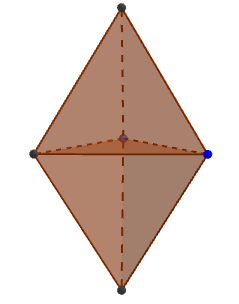
\includegraphics[scale=0.5]{double_tetrahedron.png}
	\end{center}
\end{figure}
\begin{prob}
	어떤 회의가 오후 6시에서 7시 사이에 시작해서 오후 9시에서 10시 사이에 끝났다. 회의 시작 시각의 시침과 분침의 위치가 바뀐 시각에 회의가 끝났다고 할 때, 시작 시각과 종료 시각을 각각 구하여라.
\end{prob}
회의 시작 시각의 시침의 위치를 $ x $, 분침의 위치를 $ y $, 이때의 분을 $ t_1 $, 회의 종료 시각의 분을 $ t_2 $라 하자($ x,y $의 단위는 rad이며, $0 \leq t_1, t_2 \leq 60$이다). 그러면 다음 식이 성립한다.
$$x=\pi+\dfrac{\pi}{360}t_1=\dfrac{\pi}{30}t_2$$
$$y=\dfrac{\pi}{30}t_1=\pi+\dfrac{\pi}{360}t_2$$
$ t_1 $과 $ t_2 $에 대한 방정식을 풀면 $ t_1=\dfrac{6840}{143}\approx47.83$, $ t_2=\dfrac{4860}{143}\approx33.99$가 나온다. 즉 회의는 $6$시 $\dfrac{6840}{143}$분에 시작하여 9시 $ \dfrac{4860}{143} $분에 끝났다. \begin{prob}
	한 원의 내부를 6개의 직선으로 분할할 수 있는 영역의 최대개수를 구하고, $n$개의 직선으로 한 원의 내부를 분할 할 수 있는 영역의 최대개수를 $n$에 관한 식으로 나타내어라.
\end{prob}
바로 점화식을 세우자. $ F(n) $을 $n$개의 직선을 그을 때 내부를 분할할 수 있는 영역의 최대개수라고 정의하자. 이 때 $F(0)=1$이다. 내부를 새로운 직선으로 분할할 때 추가적으로 생성되는 구역의 수는 \emph{새로 그은 직선과 교차한 직선의 수(단, 이 때 3개 이상의 직선이 한 점에서 만나면 안 된다)+1}이다. 내부 안에 직선이 $n$개 있을 때 새로운 직선을 하나 그으면 최대 $ n+1 $개의 구역이 생성되므로 $F(n+1)=n+1+F(n)$이 성립한다. 그러므로 점화식을 풀면 $ F(n)=\dfrac{n(n+1)}{2}+1, n\geq0 $이 된다. 이 때 $F(6)$은 22가 된다.\\
\\
\end{document}